% !TEX encoding = UTF-8 Unicode 
% !TEX root = praca.tex

\chapter*{Badania}

W ninjejszym rozdziale przedstawimy wyniki badań mających na celu porównanie różnych metod XAI stosowanych do wyjaśniania decyzji modeli głębokiego uczenia w kontekście klasyfikacji obrazów.
W badaniach wykozystano LIME, SHAP oraz GradCAM, aby zrozumieć, w jaki sposób te techniki różnią się pod względem generowanych wyjaśnień, dokładności oraz interpretowalności.

Analiza porównawcza została przeprowadzona w oparciu o kilka kluczowych kryteriów:
\begin{itemize}
  \item Średnia redukcja pewności
  \item Średni procentowy wzrost pewności
  \item IoU
\end{itemize}
Podczas badań każdy z powyższych kryteriów został dokładnie oceniony i zanalizowany, aby uzyskać pełny obraz mocnych i słabych stron poszczególnych metod XAI.
Przedstawione wyniki mają na celu dostarczenie wwglądu w to, jak różne techniki wyjaśniania modeli mogą być stosowane w praktyce raz jak wybrać odpowiednią metodę w zależności od konkretnych wymagań aplikacji.

\section*{Analiza porównawcza spójności wyjaśnień}
W tej sekcji przeprowadzimy analizę spójności wyjaśnień generowanych przez różne metody XAI: LIME, SHAP i GradCAM.
Naszym celem jest ocena, jak bardzo wyjaśnienia nakładają się na siebie oraz jak różne techniki identyfikują istotne cechy obrazu.

W celu oceny spójności wyjaśnień, każda z metod XAI została użyta do wygenerowania wyjjaśnień dla tego samego zestawu obrazów.
Wyniki były przedstwaione za pomocą metryki IoU, która mierzy stopień pokrycia się regionów uznawanych za istotne przez różne metody.

LIME vs SHAP
\begin{figure}
  \centering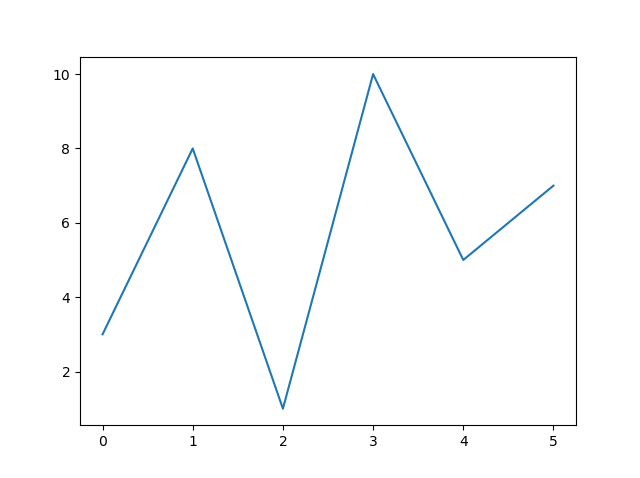
\includegraphics[width=.6\textwidth]{images/example}
\caption{Sieć dokera \cite{docker_compose_reference}}  \label{rys:network}
\end{figure}

LIME vs GradCAM
\begin{figure}
  \centering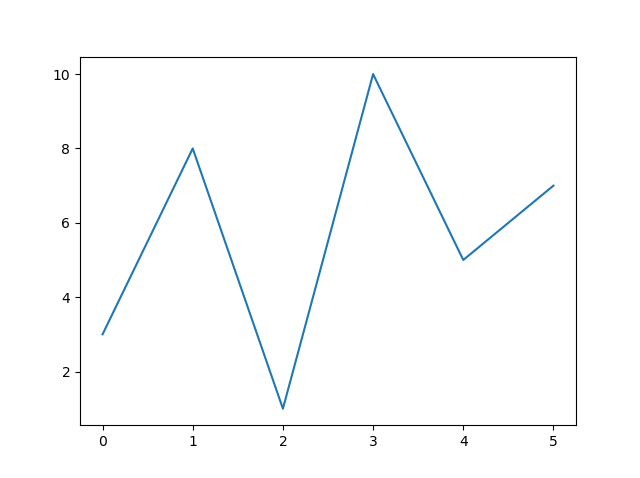
\includegraphics[width=.6\textwidth]{images/example}
\caption{Sieć dokera \cite{docker_compose_reference}}  \label{rys:network}
\end{figure}

SHAP vs GradCAM
\begin{figure}
  \centering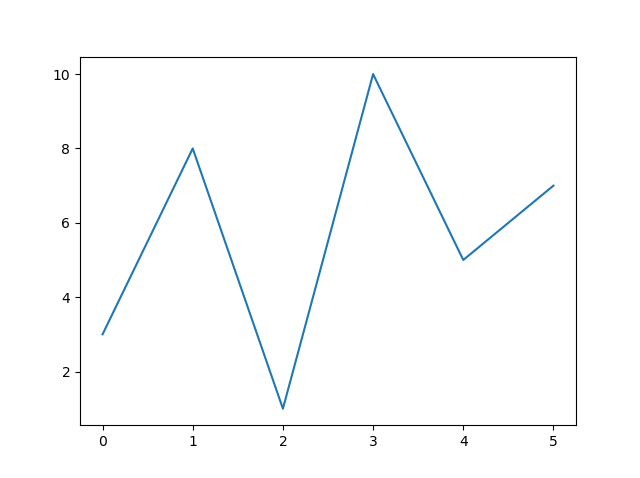
\includegraphics[width=.6\textwidth]{images/example}
\caption{Sieć dokera \cite{docker_compose_reference}}  \label{rys:network}
\end{figure}

Jak widać spójność jest ...

Aby dokładniej zrozumieć, spójność wyjaśnień, możemy przeprowadzić te same badania dzieląc wyniki również na kategorie danych:
\begin{itemize}
  \item Dog
  \item Bird
  \item Vehicle
  \item Reptile
  \item Carnivore
  \item Insect
  \item Instrument
  \item Primate
  \item Fish
\end{itemize}

\begin{figure}
  \centering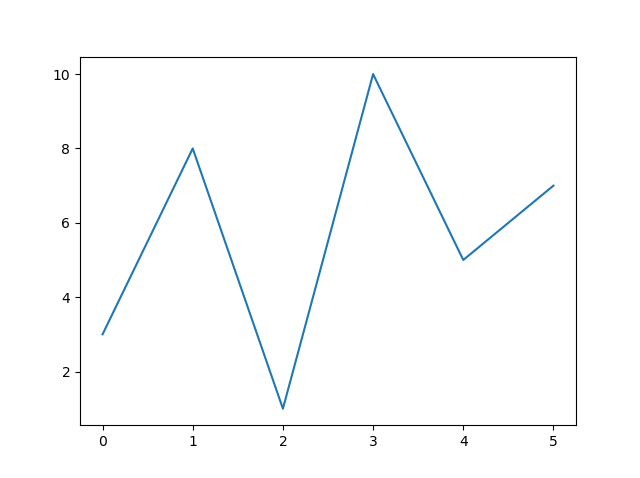
\includegraphics[width=.6\textwidth]{images/example}
\caption{Sieć dokera \cite{docker_compose_reference}}  \label{rys:network}
\end{figure}
\begin{figure}
  \centering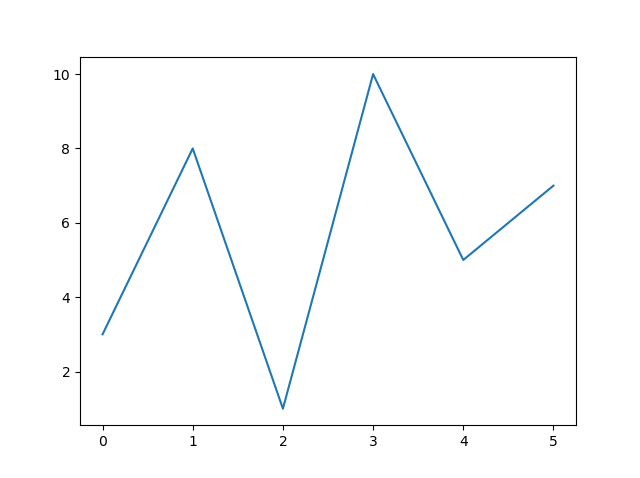
\includegraphics[width=.6\textwidth]{images/example}
\caption{Sieć dokera \cite{docker_compose_reference}}  \label{rys:network}
\end{figure}
\begin{figure}
  \centering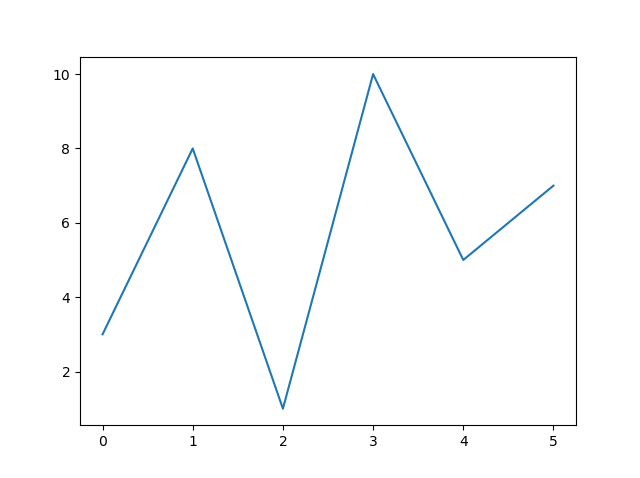
\includegraphics[width=.6\textwidth]{images/example}
\caption{Sieć dokera \cite{docker_compose_reference}}  \label{rys:network}
\end{figure}
\begin{figure}
  \centering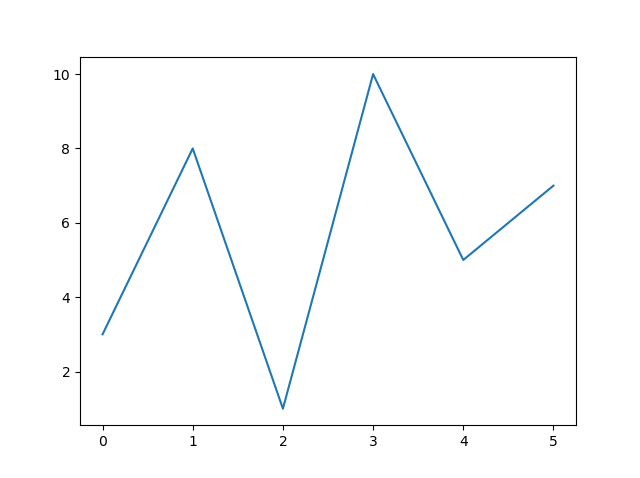
\includegraphics[width=.6\textwidth]{images/example}
\caption{Sieć dokera \cite{docker_compose_reference}}  \label{rys:network}
\end{figure}
\begin{figure}
  \centering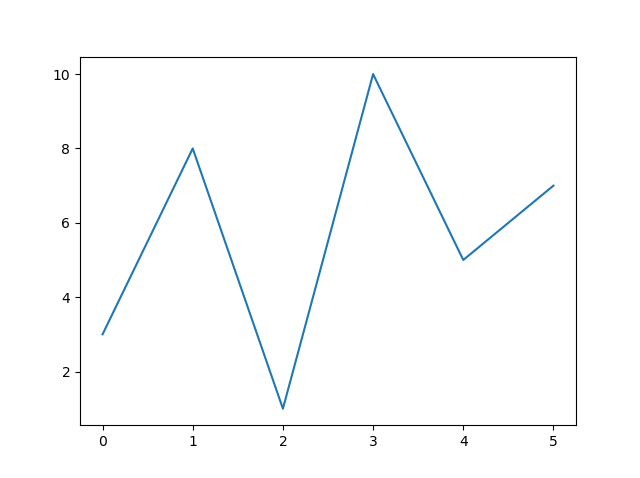
\includegraphics[width=.6\textwidth]{images/example}
\caption{Sieć dokera \cite{docker_compose_reference}}  \label{rys:network}
\end{figure}
\begin{figure}
  \centering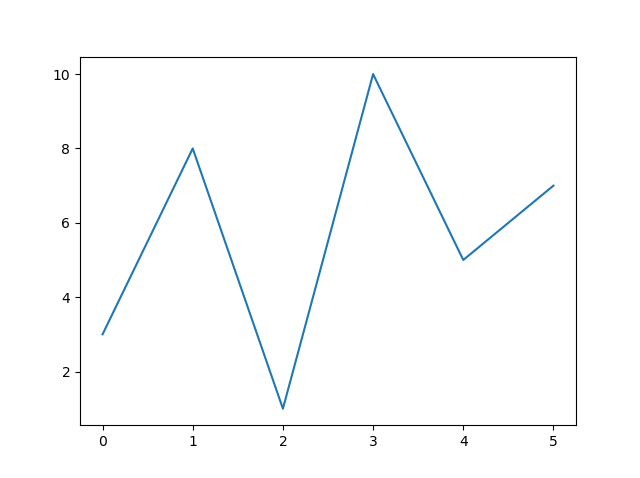
\includegraphics[width=.6\textwidth]{images/example}
\caption{Sieć dokera \cite{docker_compose_reference}}  \label{rys:network}
\end{figure}
\begin{figure}
  \centering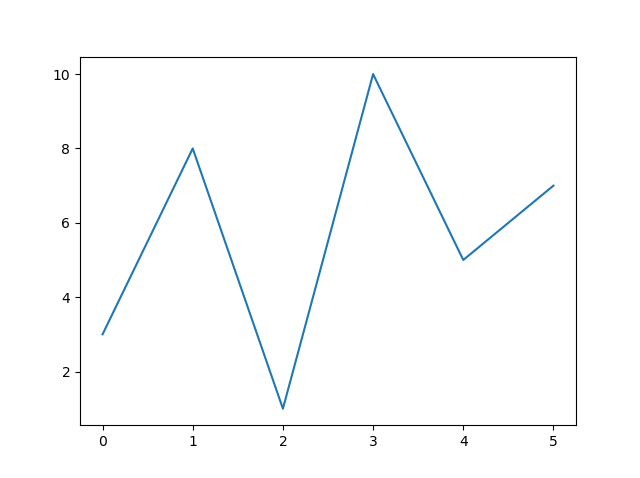
\includegraphics[width=.6\textwidth]{images/example}
\caption{Sieć dokera \cite{docker_compose_reference}}  \label{rys:network}
\end{figure}
\begin{figure}
  \centering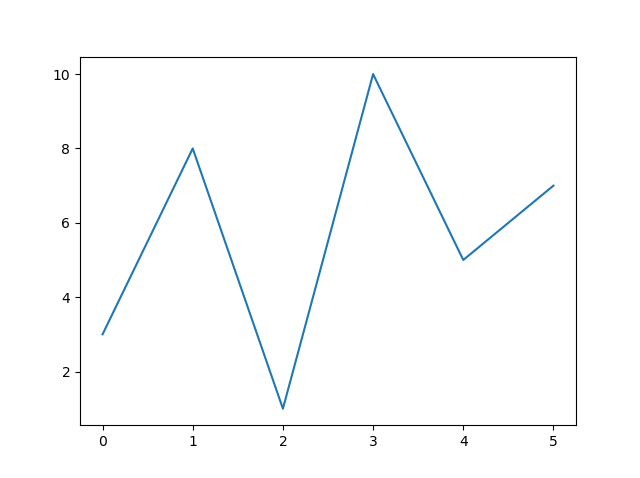
\includegraphics[width=.6\textwidth]{images/example}
\caption{Sieć dokera \cite{docker_compose_reference}}  \label{rys:network}
\end{figure}
\begin{figure}
  \centering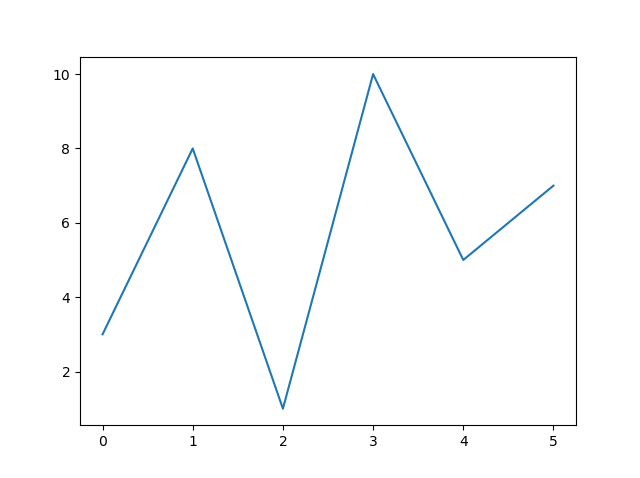
\includegraphics[width=.6\textwidth]{images/example}
\caption{Sieć dokera \cite{docker_compose_reference}}  \label{rys:network}
\end{figure}

Jak widać ...

\section*{Analiza porównacza wyjaśnień}
W tej sekcji przeprowadzimy analizę porównawcą wyjaśnień generowanych przez różne metody XAI: LIME, SHAP i GradCAM.
Oceny dokonamy na podstawie Iou oraz zmian pewności modelu.
Analiza zostaine przeprowadzona na całym zbiorze danych, a następnie z podziełem na kategorie obrazów oraz w zależności od wielkości obiektów.

/textbf{Analiza na całym zbiorze danych}.
W tej części przeprowadzimy analizę porównawczą metod XAI na całym zbiorze danych.
Skupimy się na ocenie Intersection over Union oraz zmianach w pewności modelu po zastosowaniu wyjaśnień. Celem jest zrozumienie, jak skutecznie każda metoda identyfikuje istotne cechy obrazu w kontekście całego zbioru.

IoU
\begin{figure}
  \centering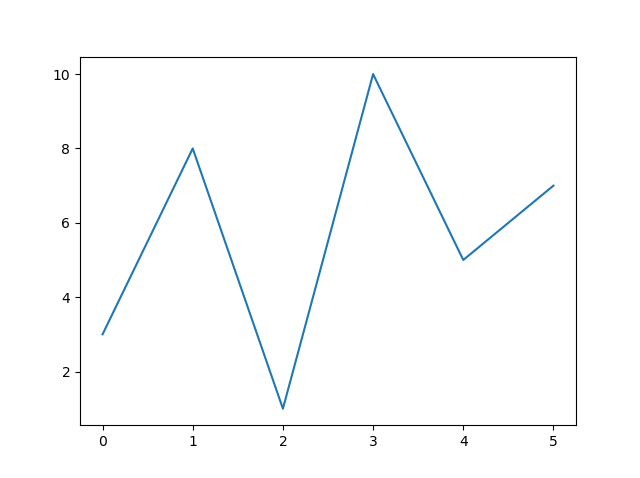
\includegraphics[width=.6\textwidth]{images/example}
\caption{Sieć dokera \cite{docker_compose_reference}}  \label{rys:network}
\end{figure}

Average Drop in Confidence
\begin{figure}
  \centering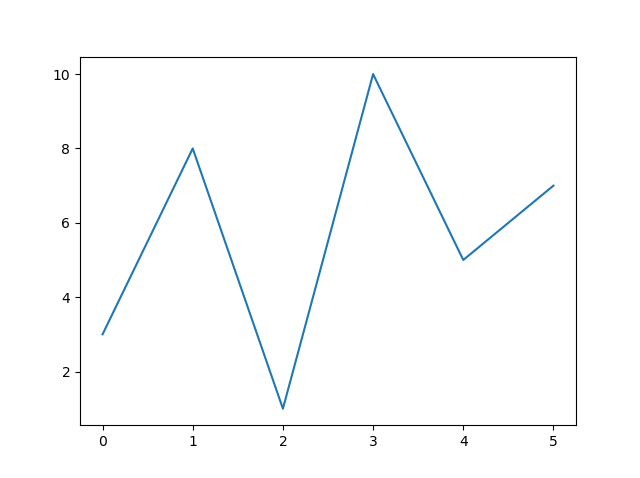
\includegraphics[width=.6\textwidth]{images/example}
\caption{Sieć dokera \cite{docker_compose_reference}}  \label{rys:network}
\end{figure}

Average Percent Increase in Confidence
\begin{figure}
  \centering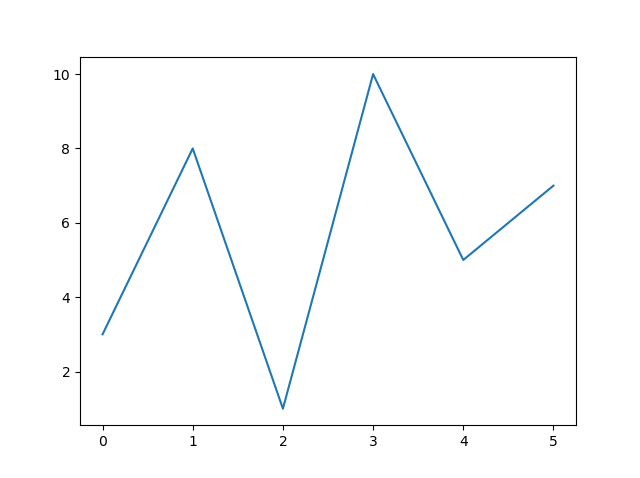
\includegraphics[width=.6\textwidth]{images/example}
\caption{Sieć dokera \cite{docker_compose_reference}}  \label{rys:network}
\end{figure}

Jak widać ...

\textbf{Analiza w zależności od klasy obrazów}.
W tej części dokonamy analizy porównawczej metod XAI z uwzględnieniem różnych kategorii obrazów.
Porównamy skuteczność wyjaśnień generowanych przez LIME, SHAP i GradCAM dla różnych klas.
Celem jest ocena, jak metody radzą sobie w kontekście specyficznych rodzajów obrazów.

IoU
\begin{figure}
  \centering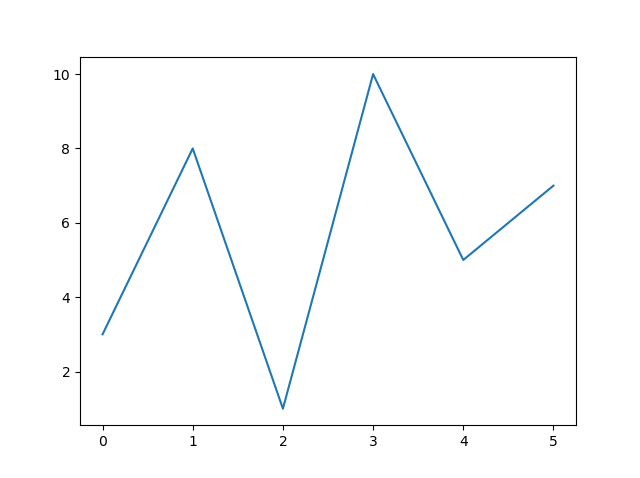
\includegraphics[width=.6\textwidth]{images/example}
\caption{Sieć dokera \cite{docker_compose_reference}}  \label{rys:network}
\end{figure}

Average Drop in Confidence
\begin{figure}
  \centering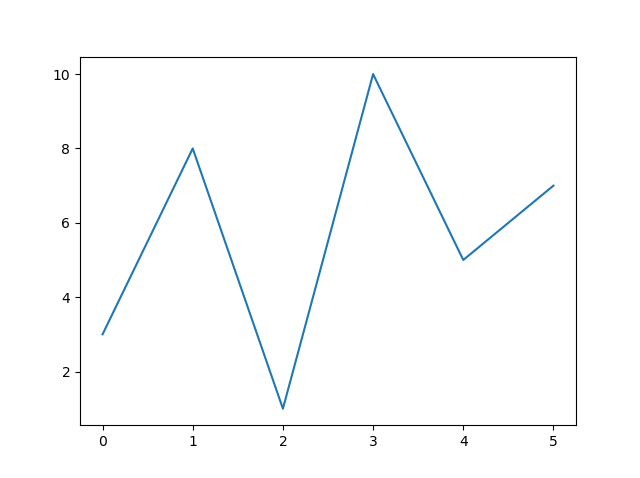
\includegraphics[width=.6\textwidth]{images/example}
\caption{Sieć dokera \cite{docker_compose_reference}}  \label{rys:network}
\end{figure}

Average Percent Increase in Confidence
\begin{figure}
  \centering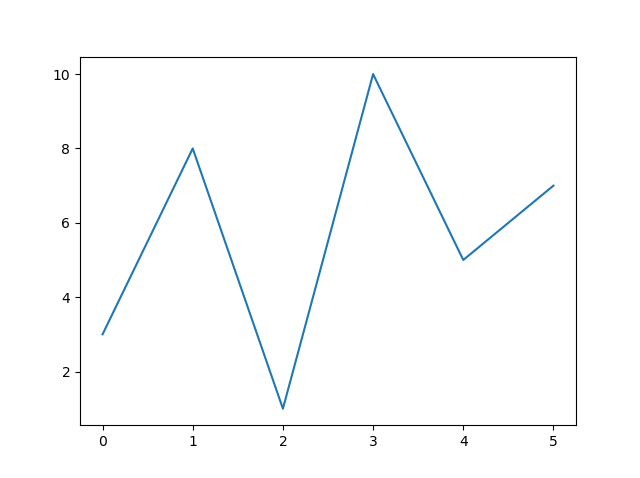
\includegraphics[width=.6\textwidth]{images/example}
\caption{Sieć dokera \cite{docker_compose_reference}}  \label{rys:network}
\end{figure}

Jak widać ...

\textbf{Analiza w zależności od wielkości obiektu}.
Przeanalizujemy teraz, jak metody XAI radzą sobie w identyfikacji istotnych cech obrazów w zależności od wielkości obiektów.
Porównamy wyniki IoU oraz zmiany pewności modelu dla małych, średnich oraz dużych obiektów.
Celem jest zrozumienie, jak wielkość obiektu wpływa na skuteczność wyjaśnień generowanych przez różne metody.
małe obiekty definiujemy jako obiekty zajmujące mniej niż 10\% obrazu, średnie mniej niż 50\%, natomiast duże to ponad 50\%.

IoU
\begin{figure}
  \centering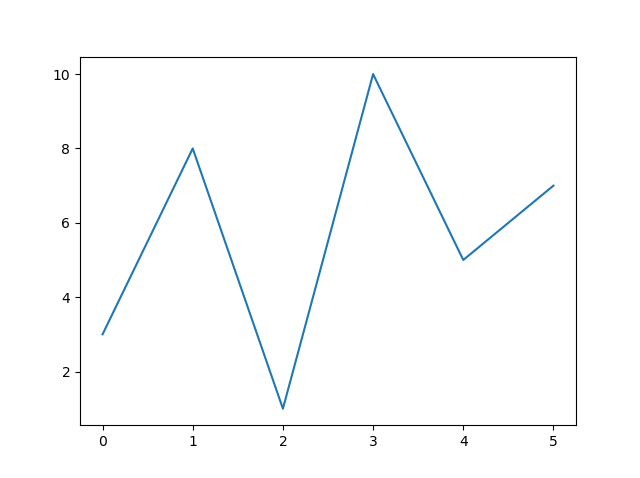
\includegraphics[width=.6\textwidth]{images/example}
\caption{Sieć dokera \cite{docker_compose_reference}}  \label{rys:network}
\end{figure}

Average Drop in Confidence
\begin{figure}
  \centering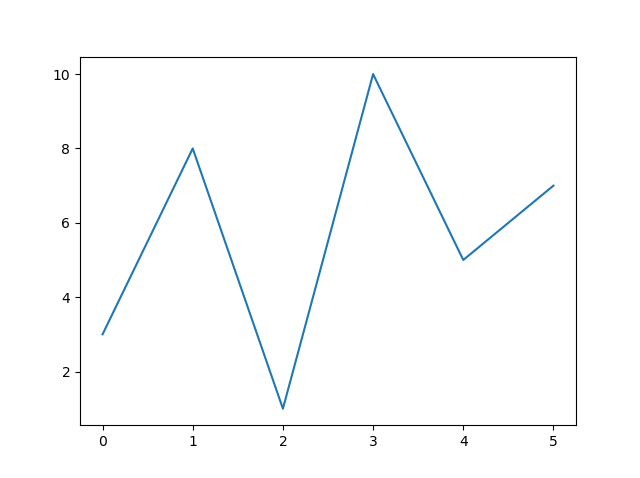
\includegraphics[width=.6\textwidth]{images/example}
\caption{Sieć dokera \cite{docker_compose_reference}}  \label{rys:network}
\end{figure}

Average Percent Increase in Confidence
\begin{figure}
  \centering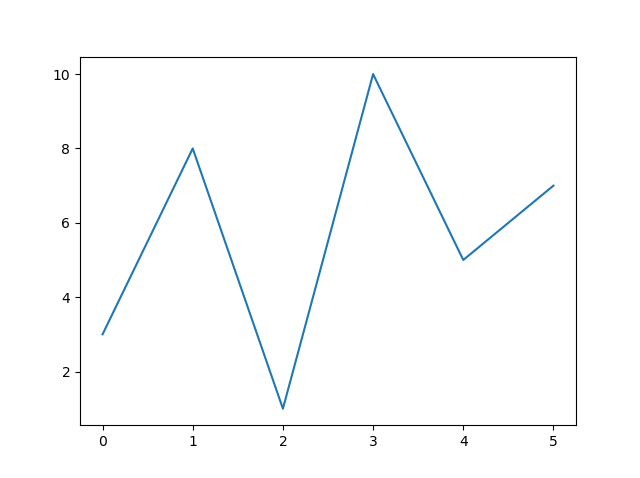
\includegraphics[width=.6\textwidth]{images/example}
\caption{Sieć dokera \cite{docker_compose_reference}}  \label{rys:network}
\end{figure}

Jak widać ...

\textbf{Wnioski}

\section*{Łączenie wyjaśnień różnych metod}
W tej sekcji przanalizujemy połączenie wyjaśnień generowanych przez różne matody XAI: LIME, SHAP i GradCAM.
Celem jest sprawdzenie, czy łączenie tych metod może dostarczyć bardziej szczegółowych lub ogólnych wyjaśnień.
Przeprowadzimy analizę na całym zbiorze danych, porównując wyniki uzyskane z połączenia wyjaśnień przez część wspólną oraz sumę obszarów

\textbf{Połączenie wyjaśnień LIME i SHAP}

\textbf{Część wspólna} - Łącząc wyjaśnienia poprzez ich część wspólną, identyfikujemy cechy, które są uznawane za istone przez obie metody.
Ten sposób połączenia ma na celu uzyskanie bardziej precyzyjnych i szczegółowych wyjaśnień, wskazując na kluczowe cechy, które są najważniejsze dla modelu.
\begin{figure}
  \centering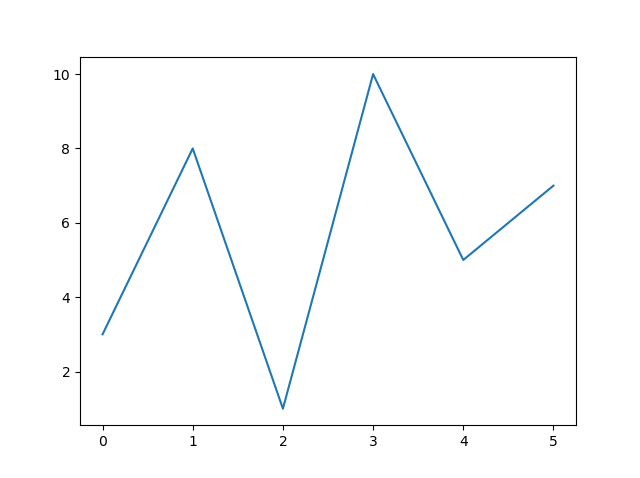
\includegraphics[width=.6\textwidth]{images/example}
\caption{Sieć dokera \cite{docker_compose_reference}}  \label{rys:network}
\end{figure}

\textbf{Suma obszarów} - Sumując obszary wyjaśnień uzyskujemy bardziej ogólne wyjaśnienia, które mogą obejmować szrszy zakres istotnych cech.
To podejście pozwala na identyfikację wszystkich potencjalnie ważnych regionów na obrazie.
\begin{figure}
  \centering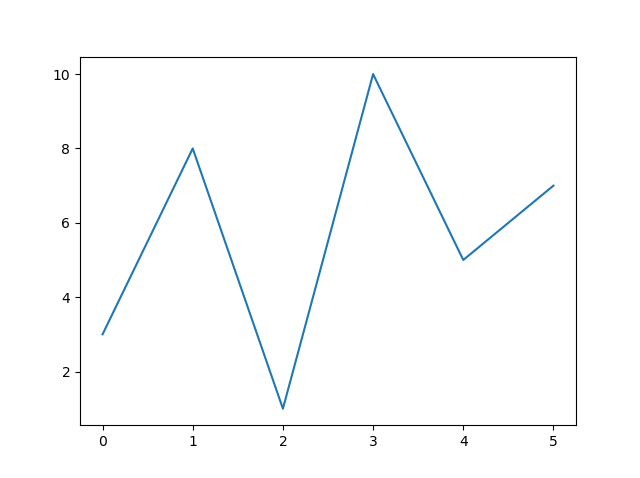
\includegraphics[width=.6\textwidth]{images/example}
\caption{Sieć dokera \cite{docker_compose_reference}}  \label{rys:network}
\end{figure}

\textbf{Połączenie wyjaśnień LIME i GradCAM}

\textbf{Część wspólna} - Łącząc wyjaśnienia poprzez ich część wspólną, identyfikujemy cechy, które są uznawane za istone przez obie metody.
Ten sposób połączenia ma na celu uzyskanie bardziej precyzyjnych i szczegółowych wyjaśnień, wskazując na kluczowe cechy, które są najważniejsze dla modelu.
\begin{figure}
  \centering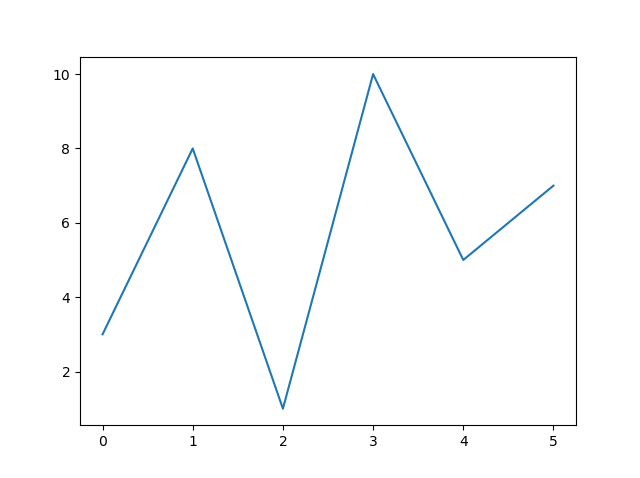
\includegraphics[width=.6\textwidth]{images/example}
\caption{Sieć dokera \cite{docker_compose_reference}}  \label{rys:network}
\end{figure}

\textbf{Suma obszarów} - Sumując obszary wyjaśnień uzyskujemy bardziej ogólne wyjaśnienia, które mogą obejmować szrszy zakres istotnych cech.
To podejście pozwala na identyfikację wszystkich potencjalnie ważnych regionów na obrazie.
\begin{figure}
  \centering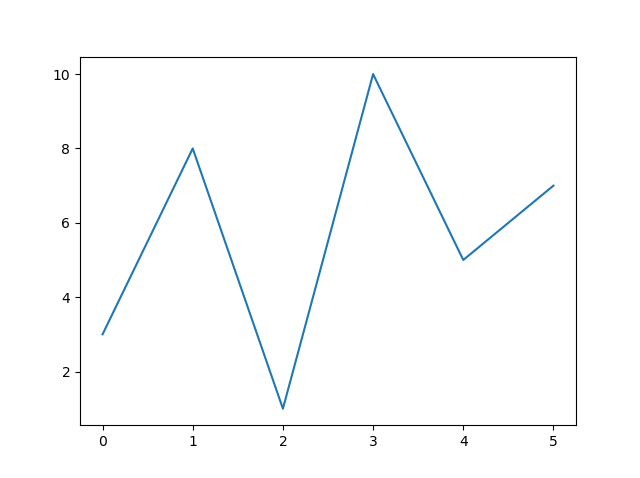
\includegraphics[width=.6\textwidth]{images/example}
\caption{Sieć dokera \cite{docker_compose_reference}}  \label{rys:network}
\end{figure}

\textbf{Połączenie wyjaśnień SHAP i GradCAM}

\textbf{Część wspólna} - Łącząc wyjaśnienia poprzez ich część wspólną, identyfikujemy cechy, które są uznawane za istone przez obie metody.
Ten sposób połączenia ma na celu uzyskanie bardziej precyzyjnych i szczegółowych wyjaśnień, wskazując na kluczowe cechy, które są najważniejsze dla modelu.
\begin{figure}
  \centering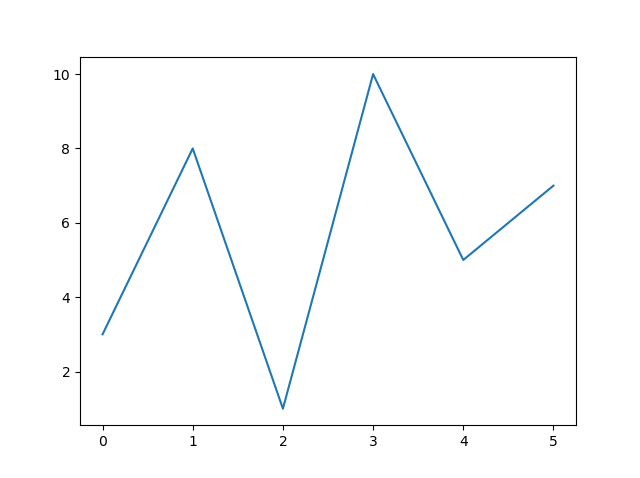
\includegraphics[width=.6\textwidth]{images/example}
\caption{Sieć dokera \cite{docker_compose_reference}}  \label{rys:network}
\end{figure}

\textbf{Suma obszarów} - Sumując obszary wyjaśnień uzyskujemy bardziej ogólne wyjaśnienia, które mogą obejmować szrszy zakres istotnych cech.
To podejście pozwala na identyfikację wszystkich potencjalnie ważnych regionów na obrazie.
\begin{figure}
  \centering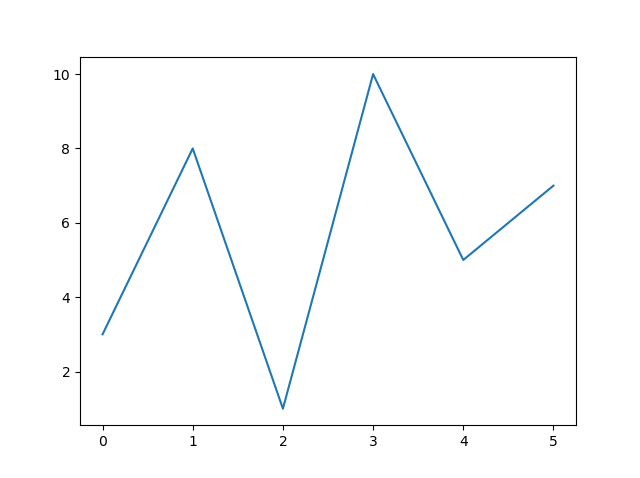
\includegraphics[width=.6\textwidth]{images/example}
\caption{Sieć dokera \cite{docker_compose_reference}}  \label{rys:network}
\end{figure}

\textbf{Połączenie wyjaśnień LIME, SHAP i GradCAM}

\textbf{Część wspólna} - Łącząc wyjaśnienia poprzez ich część wspólną, identyfikujemy cechy, które są uznawane za istone przez obie metody.
Ten sposób połączenia ma na celu uzyskanie bardziej precyzyjnych i szczegółowych wyjaśnień, wskazując na kluczowe cechy, które są najważniejsze dla modelu.
\begin{figure}
  \centering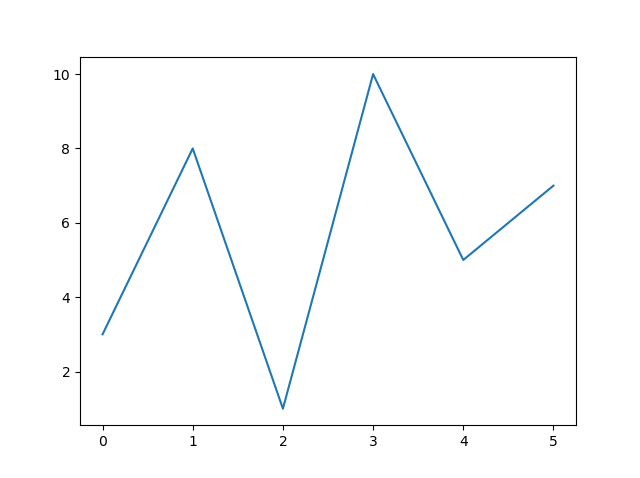
\includegraphics[width=.6\textwidth]{images/example}
\caption{Sieć dokera \cite{docker_compose_reference}}  \label{rys:network}
\end{figure}

\textbf{Suma obszarów} - Sumując obszary wyjaśnień uzyskujemy bardziej ogólne wyjaśnienia, które mogą obejmować szrszy zakres istotnych cech.
To podejście pozwala na identyfikację wszystkich potencjalnie ważnych regionów na obrazie.
\begin{figure}
  \centering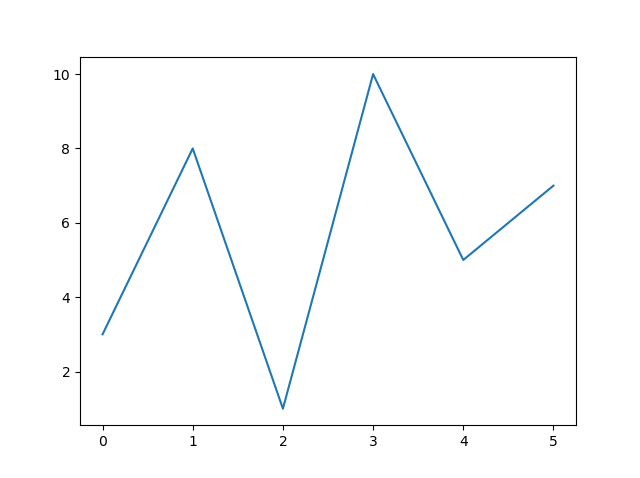
\includegraphics[width=.6\textwidth]{images/example}
\caption{Sieć dokera \cite{docker_compose_reference}}  \label{rys:network}
\end{figure}

\section*{Porównanie z innym zbiorem danych}

Może jakieś porównanie ze specyficznymi zbiorami.

\section*{Porównanie z innymi modelami klasyfikacji obrazów}
W tej sekcji porównamy wyjaśnienia generowane przez XAI dla różnych modeli klasyfikacji obrazów.
Wyjaśnienia te mogą się różnić w zależności od zastosowanego modelu, co wpływa na interpretację wyników i zrozumienie działania modelu.

Jednm z głównych aspektów, który należy uwzględnić przy porównywaniu wyjaśnień z różnych modeli, jest rozdzielczość wyjaśnień generowanych przez GradCAM.
Rozdzielczość ta zależy od wymiarów wyjściowych warstw konwolucyjnych modelu.
W przypdaku modeli o różnych architekturach, takich jak ResNet, VGG czy Inception, wyjściowe wymiary warstw konwolucyjnych mogą się znacznie różnić, co prowadzi do wyjaśnień o różnych pozimach szczegółowości.

W celu oceny spójności wyjaśnień, każda z metod XAI została użyta do wygenerowania wyjjaśnień dla tego samego zestawu obrazów.
Wyniki były przedstwaione za pomocą metryki IoU, która mierzy stopień pokrycia się regionów uznawanych za istotne przez różne metody.

LIME vs SHAP
\begin{figure}
  \centering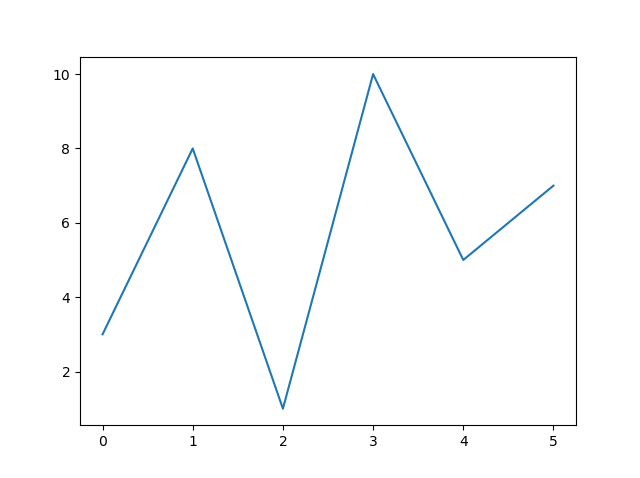
\includegraphics[width=.6\textwidth]{images/example}
\caption{Sieć dokera \cite{docker_compose_reference}}  \label{rys:network}
\end{figure}

LIME vs GradCAM
\begin{figure}
  \centering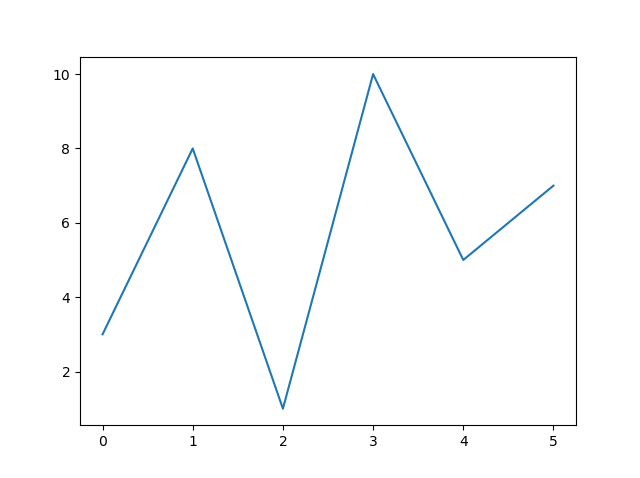
\includegraphics[width=.6\textwidth]{images/example}
\caption{Sieć dokera \cite{docker_compose_reference}}  \label{rys:network}
\end{figure}

SHAP vs GradCAM
\begin{figure}
  \centering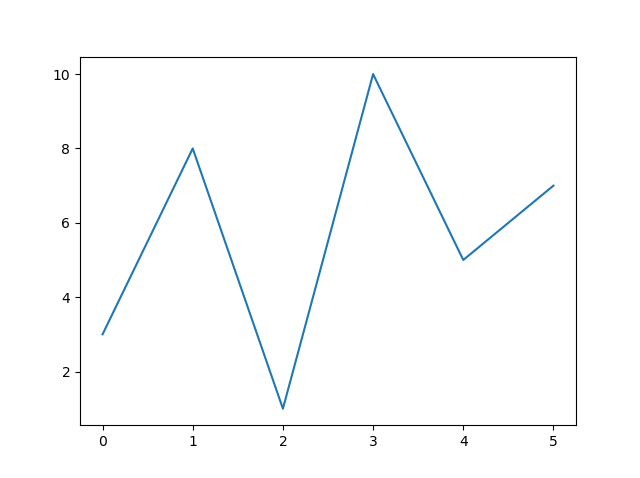
\includegraphics[width=.6\textwidth]{images/example}
\caption{Sieć dokera \cite{docker_compose_reference}}  \label{rys:network}
\end{figure}

Jak widać spójność jest ...

W tej części przeprowadzimy analizę porównawczą metod XAI na całym zbiorze danych.
Skupimy się na ocenie Intersection over Union oraz zmianach w pewności modelu po zastosowaniu wyjaśnień. Celem jest zrozumienie, jak skutecznie każda metoda identyfikuje istotne cechy obrazu w kontekście całego zbioru.

IoU
\begin{figure}
  \centering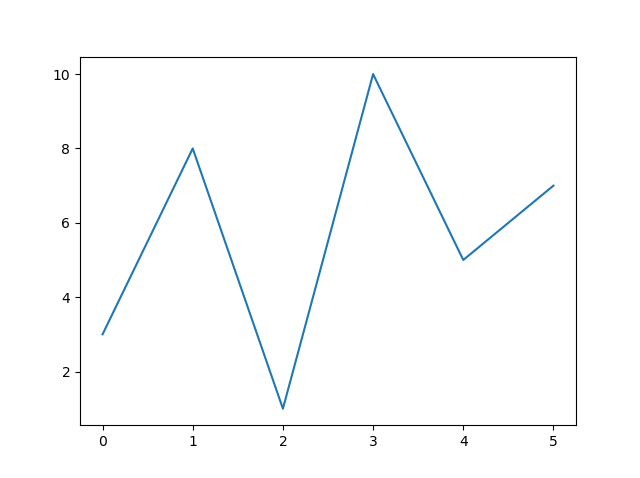
\includegraphics[width=.6\textwidth]{images/example}
\caption{Sieć dokera \cite{docker_compose_reference}}  \label{rys:network}
\end{figure}

Average Drop in Confidence
\begin{figure}
  \centering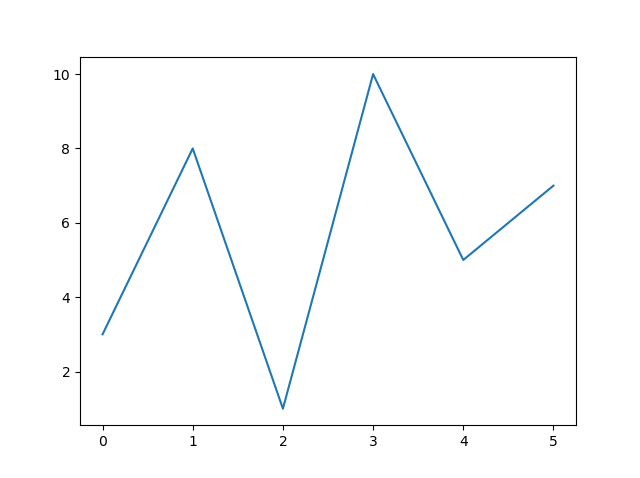
\includegraphics[width=.6\textwidth]{images/example}
\caption{Sieć dokera \cite{docker_compose_reference}}  \label{rys:network}
\end{figure}

Average Percent Increase in Confidence
\begin{figure}
  \centering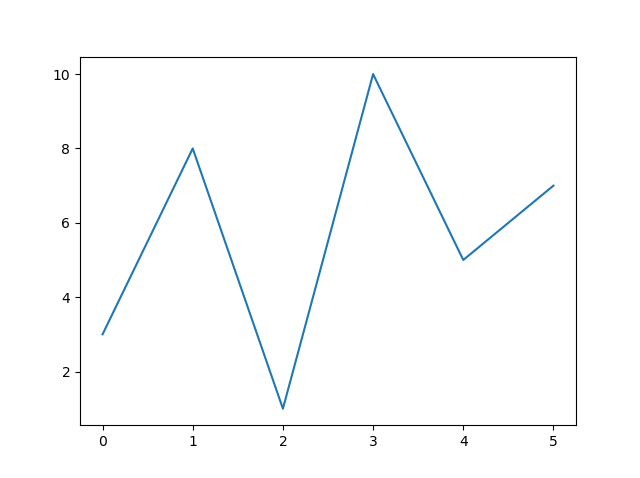
\includegraphics[width=.6\textwidth]{images/example}
\caption{Sieć dokera \cite{docker_compose_reference}}  \label{rys:network}
\end{figure}

Jak widać ...

\section*{Ocena poszczegóĺnych algorytmów}
Ocena poszczególnych algorytmów.
Porównanie wyników metod pod kątem ich zdolności do dostarczania zrozumiałych i precyzyjnych wyjaśnień.
Słabe i mocne strony każdej metody.
Czas wykonania eksperymentów oraz złożoność obliczeniowa

